\chapter{Design}
\section{Visuals}
The interface will utilize a dual-theme approach: a light mode with a subtle dotted background to enhance readability during daytime, while a dark mode will reduce eye strain for those working later hours. With more employees choosing flexible working options due to the shift to working from home, it is important for users to reduce the amount of blue light in the evening \parencite{cipd2023flexible}. The primary colour, purple, aligns with the Royal College of Radiologists' (RCR’s) branding, creating a professional and cohesive aesthetic. Red will be used selectively for critical actions like logout and reject buttons, drawing immediate attention.

Clean, sans-serif fonts will be used for easy legibility, and consistent layout structures will be maintained, even across different screens, to support muscle memory and navigability. The layout will take some inspiration from the recent trend of Bento UI, where information is broken into separate cards of a single category. This design style is ideal for a project that requires the users to have access to so much data, because it allows for compartmentalising information effectively. 'isms' such as Neumorphism and Glassmorphism will be used sparingly. Whilst they add depth to the design, allowing users to differentiate between elements we want them to focus on most, they can also be distracting, and appear unprofessional when overused.

There are countless other design choices that go beyond this, the majority of which are applied subconsciously. My personal style is heavily influenced by \citetitle{muller-brockmann_grid_1981} by \textcite{muller-brockmann_grid_1981} and the more recent \citetitle{wathan_refactoring_2018} by \textcite{wathan_refactoring_2018}.
\section{Frameworks}
\subsection{Django} \label{Django}
Django is chosen for its comprehensive feature set that simplifies many web development tasks thanks to its "batteries-included" design. Django’s ORM (Object-Relational Mapping) system will be used to manage database operations much more efficiently than through direct SQL, which is crucial given the complex data relationships in the RCR’s processes. Its built-in security features as less essential as it will have limited internet access, however tools such as SQL Injection protection and Cross-Site Scripting (XSS) protection are still paramount.

To turn Django into an API, Django-Ninja will be implemented for its exceptional speed and ease of use. The use of Pydantic with Django-Ninja ensures strong type checking, significantly reducing the risk of bugs that are usually common in Python and JavaScript. Its integration with OpenAPIs automatic documentation allows us to test the API in SwaggerUI before writing any frontend code, and can even be used to transfer schemas from backend to frontend. This library also supports Django's asynchronous capabilities. However, it will not be used in this project as the frequency of requests is not high enough to warrant the additional complexity, though it leaves room for scalability if needed.

Django-Ninja-JWT, built on top of Django-Ninja-Extra, provides JWT (JSON Web Tokens) authentication, essential for secure API access in our application. This feature allows for stateless authentication, making it easier to manage sessions in a distributed environment where the RCR's data may need to be accessed securely across multiple locations. The JWTs will be stored securely using HTTP-only cookies, configured with strict properties to prevent unauthorized access. It also eliminates the need to handle CSRF tokens in Django, though SvelteKit already handles this by default.

\subsubsection{Alternative API Framework}
\begin{figure}[h]
\centering
\frame{\includegraphics[width=\linewidth]{images/Django-Ninja-speed.png}}
\vspace{-15pt}
\caption{Various Django API framework speeds}
\vspace{-10pt}
\caption*{\parencite{vitaliy_kucheryaviy_django_2024}
\label{fig:Django-Ninja-speed}}
\vspace{-5pt}
\end{figure}
Django Rest Framework (DRF) is the most popular choice for building APIs in Django. However, it lacks the type hints, Pydantic integration, simplicity, and automatic documentation of Django-Ninja. Figure \ref{fig:Django-Ninja-speed} shows the enormous speed difference between the two, even when concurrency is not used.

\subsubsection{PyTransitions}
The Python 'transitions' library for state management of JDs. State machines are crucial for enforcing the rules and transitions of a workflow's various stages, and ensure that each job description progresses through its lifecycle in a controlled, traceable manner, preventing errors and ensuring consistency. It also gives users the ability to track the progress of each JD visually by generating state machine diagrams based on the current state in relation to others.

\subsection{SvelteKit} \label{SvelteKit}
You may have noticed that there is no dedicated Backend and Frontend section. This is because SvelteKit in itself is a full-stack framework. There are a number of reasons for this, most notably that the frontend, Svelte, and backend are extremely closely integrated and are essentially one entity. This allows us to have features such as a file based routing system, simplified state management, and much more. This is a key advantage of SvelteKit over other frameworks, as it allows for a more seamless development experience. The performance is also superb, as it compiles to vanilla JavaScript and removes the overhead of the virtual DOM - though the performance difference with a framework such as Vue3 is negligible. On low-end devices or poor network connections however, which can be common where organisations are underfunded, adaptive loading and progressive enhancement can make a huge difference. As discussed in \ref{Background}, is extremely important that this system is as accessible as possible, especially to Trusts that need it most, as a large part of the National Health Service depends on this process. 

The use of a 'second backend' allows a more modular design. By allowing Django to focus exclusively on serving and managing the database, SvelteKit's backend can focus on rendering the frontend, handling user interactions, and manipulating form data into a cleaner format. This leaves Svelte to handle the UI with data in a format easiest for HTML to display. 

\begin{figure}[h]
\centering
\frame{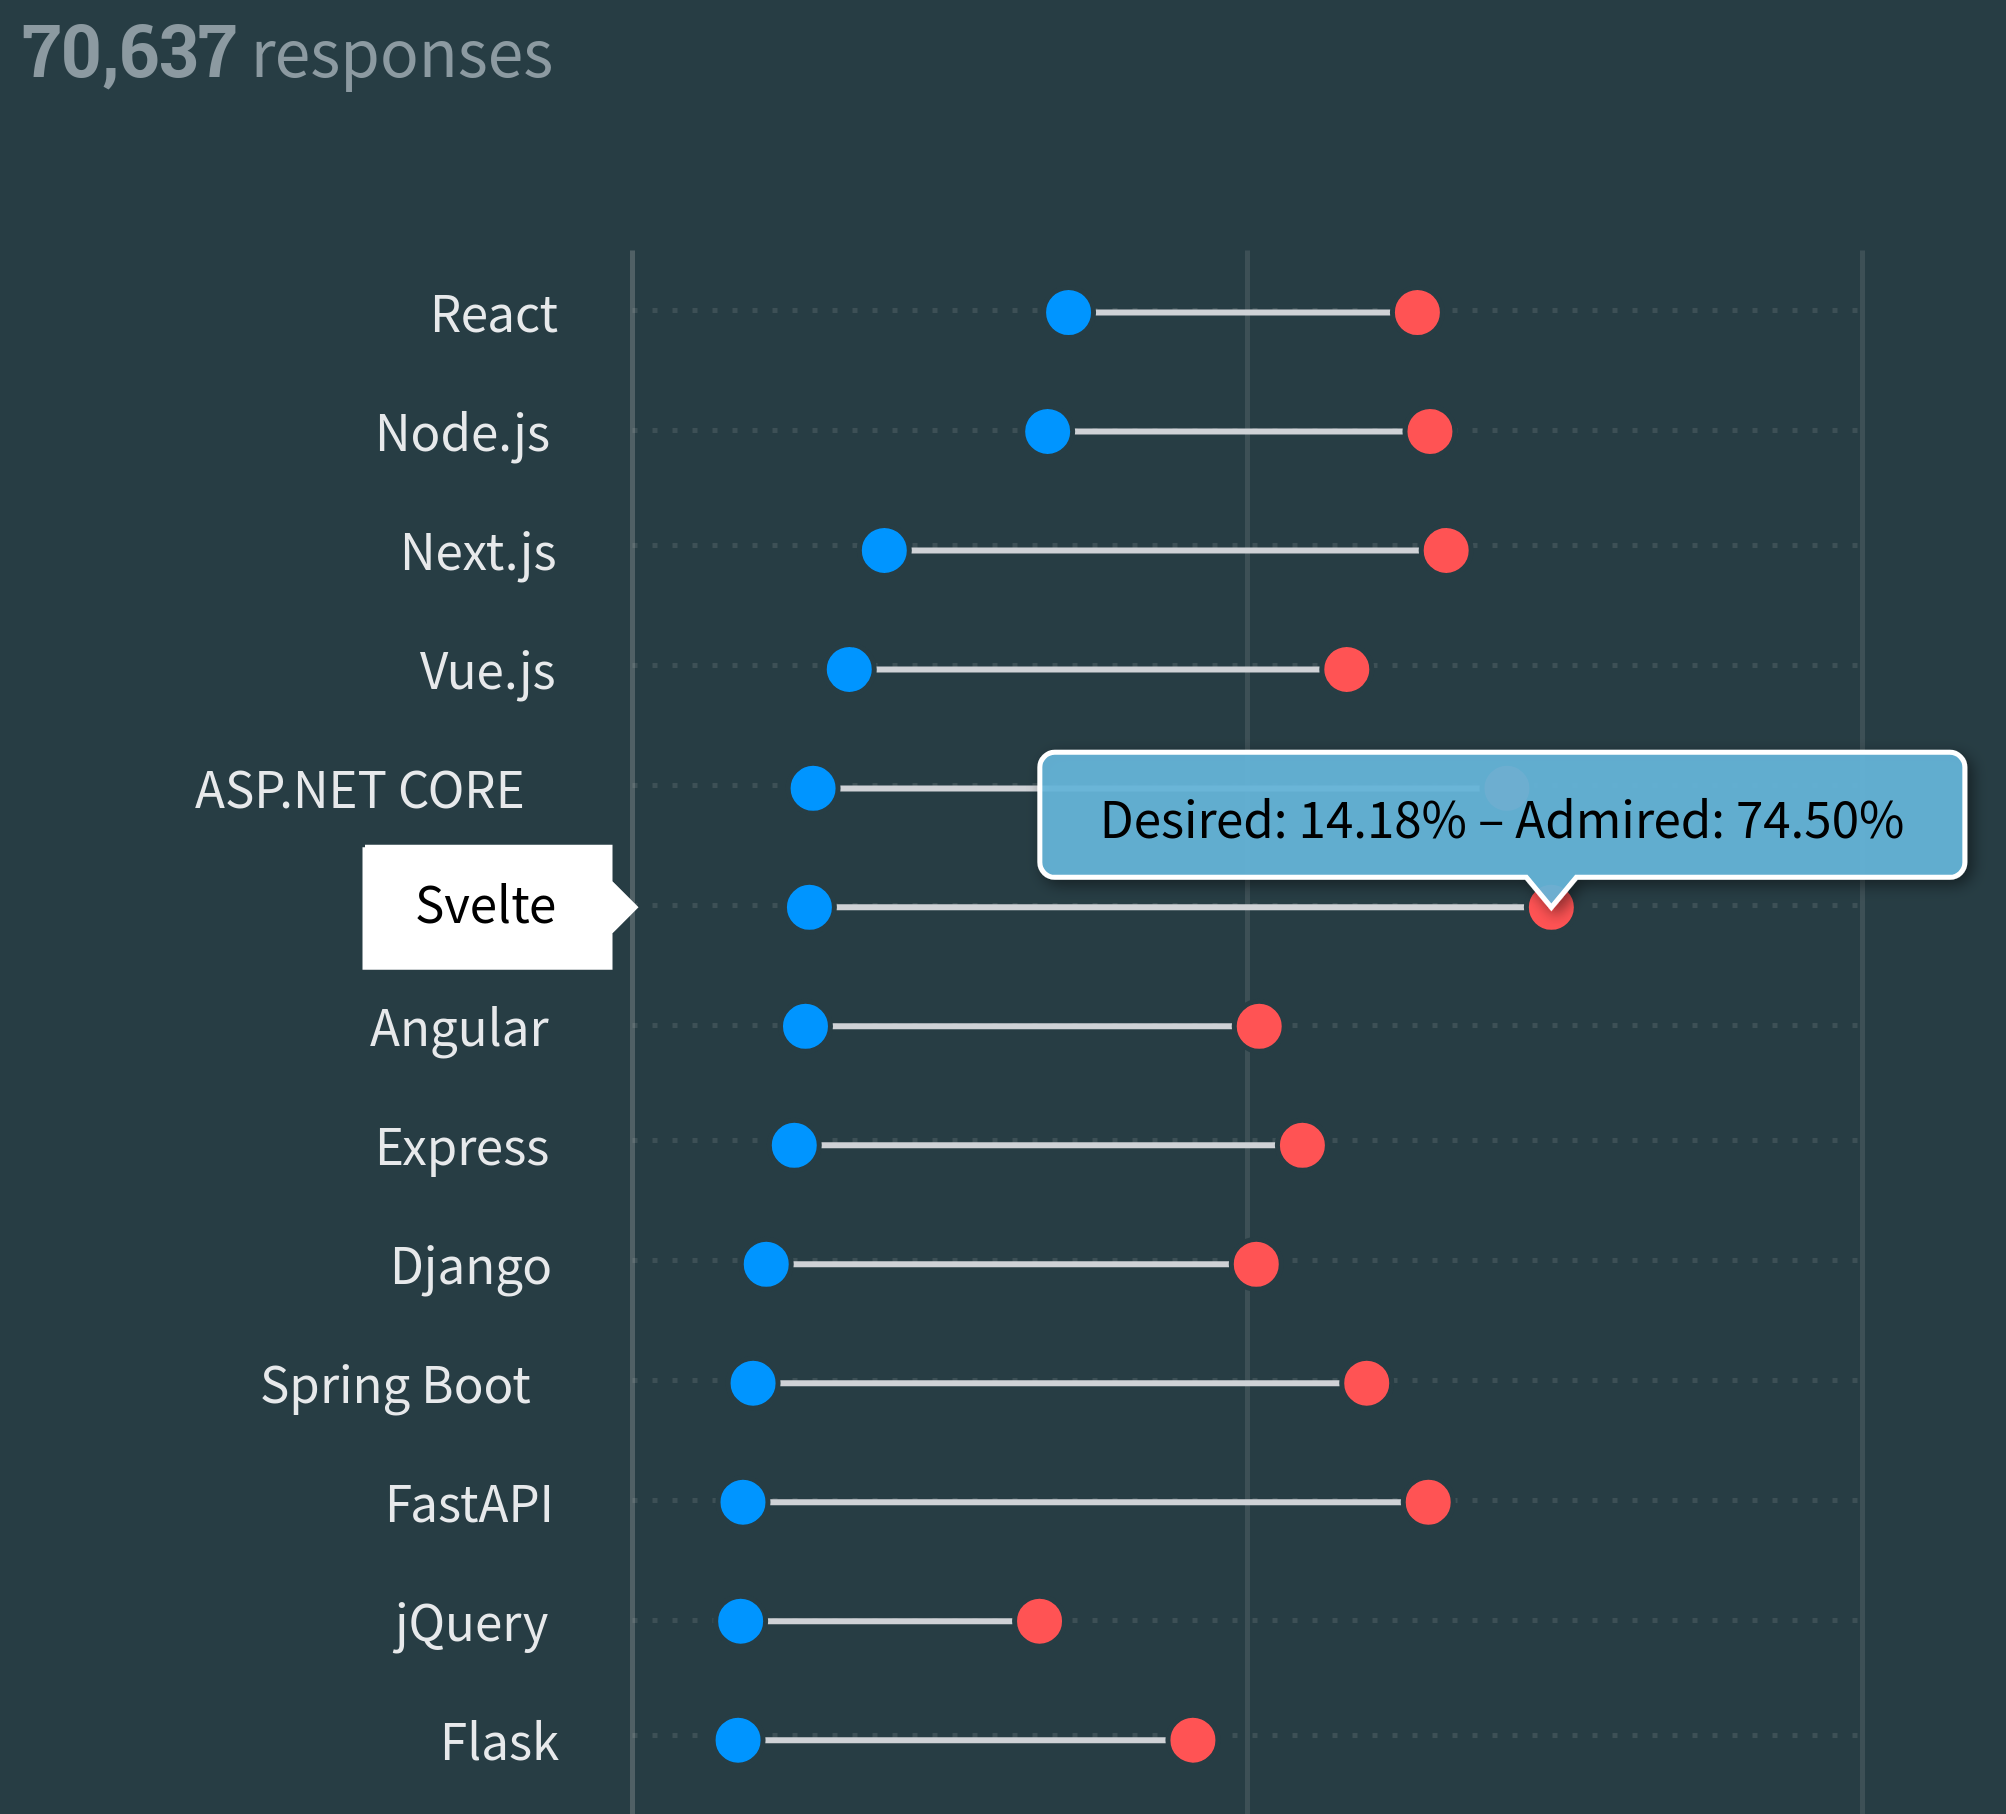
\includegraphics[width=0.8\linewidth]{images/svelte.png}}
\caption{Svelte ranking}
\vspace{-10pt}
\caption*{Consistently one of the most admired web frameworks, scoring second highest in 2023}
\vspace{-10pt}
\caption*{\parencite{noauthor_stack_nodate}}
\label{fig:svelte}
\vspace{-5pt}
\end{figure}

\subsubsection{Libraries}
TypeScript will allow strict typing, just like in the Django-Ninja Schema. As discussed in \ref{Django}, OpenAPI-Typescript allows us to import this schema into SvelteKit, providing type safety and autocompletion without having to rewrite all of the types in a completely different language. This ensures that the frontend and backend development environment are always in sync, reducing the likelihood of errors and inconsistencies. 

These types will be used in requests with Axios, which will be responsible for communicating with Django. It is easier to work with than native JavaScript's Fetch as it is more readable with less boilerplate, but more importantly, it has automatic JSON transformation which will be essential for handling the complicated forms that will be built. A custom API library will be built on top to abstract this code even more, which can turn over 10 lines of code into a single function call. These functions can be used anywhere in the program, and since the same data is likely to be used in multiple different pages, it also removes the need to repeat code. Lastly, by having a single source of truth for the API, not only is it easier to make changes to the API without having to change every single page that uses it, but it also reduces the changes of bugs due to typos to almost zero.

Postmark is an email delivery service which will be used for email verification and notifications. It is preferred over self-hosted emailing, as those are usually blocked as spam by all major email services, but still allows us to use our own custom domains through DKIM and Return-Path DNS records. It features a very easy to use API, and a very high deliverability rate, as all developers have to be approved by Postmark through a manually reviewed form.

shadcn-svelte is not so much a library, but rather a set of re-usable components build on top of a number of other libraries. It allows us to keep a consistent design across the entire application, and reduce time spent on building basic parts of the UI. This does however mean that the multitude of libraries it is built on top of have to be learnt and a deep understanding of the documentation is a requirement. These libraries will include; Svelte Headless Table for data tables. Formsnap, Superforms and Zod for form processing and validation. Bits UI (built on top of Melt UI) for the majority of the components. And TailwindCSS for styling and positioning. The form libraries are particularly important. While forms are one of the common features on the web, they are also one of the most complex - and this project is almost entirely based on large, complicated, and dynamic forms.

Luckily this setup will allow us to build well-structured and semantically correct forms, with client and server side validation. There are also Accessible Rich Internet Application (ARIA) attributes and proper labels for screen readers to make the website accessible to all users. Lastly they are generally easy to use and can be navigated exclusively with a keyboard. 

\section{Deployment}
For the purposes of this project, the website will be deployed on a Linux server with Nginx, Gunicorn, and Node with its respective SvelteKit adaptor. Nginx will be used as the reverse proxy and HTTP server, along with Cerbot for automatic SSL certificates. The Django admin panel may also be exposed publicly to allow access for RCR Employees working from home. Gunicorn will be used with multiple workers to handle multiple requests at once, as opposed to using Django-Ninja's asynchronous features. Node.js for SSR will improve load times and SEO. Though the latter is not as important, assuming the website will be a link in an existing RCR webpage, it will still help users searching for the website avoid multiple navigations. This may reduce the number of phone calls and emails received attempting to find the correct RCR department.


\section{File Structure} \label{File Structure}
\begin{figure}[h]
\centering
\frame{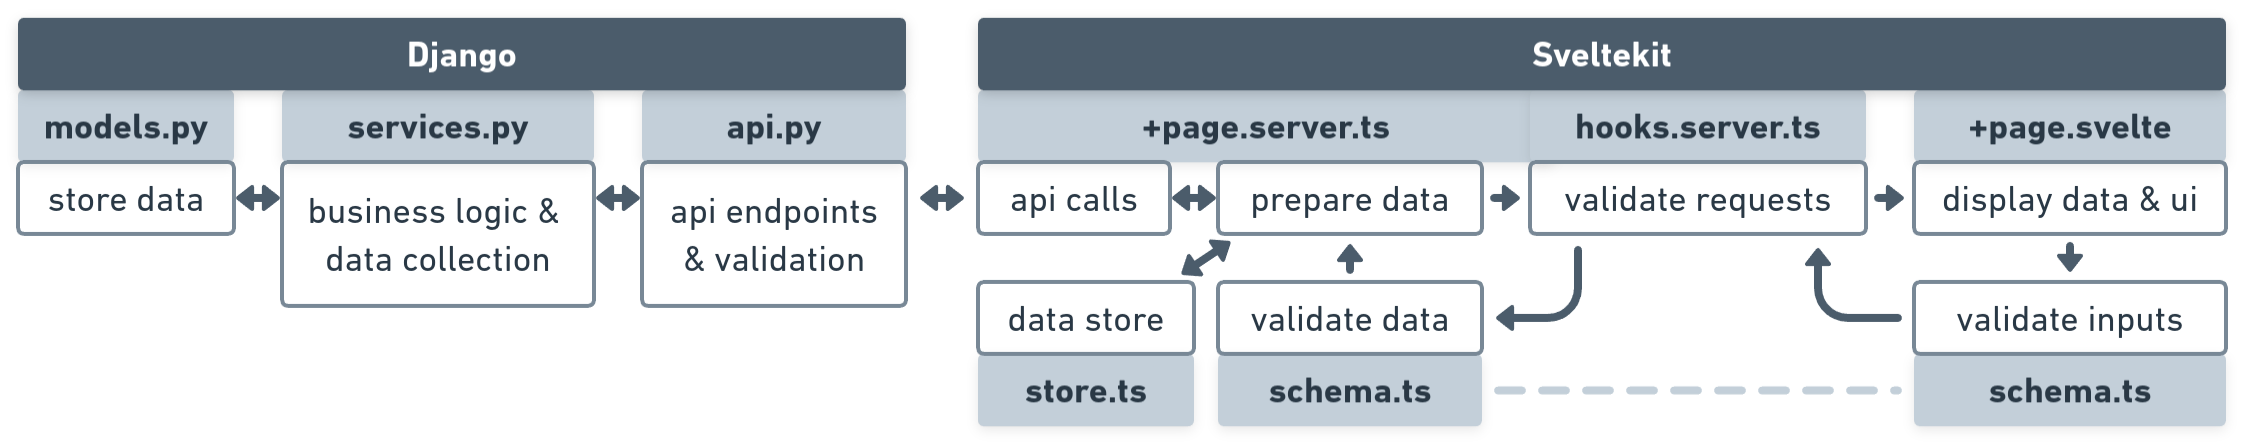
\includegraphics[width=\linewidth]{images/design.png}}
\vspace{-20pt}
\caption{System file structure}
\label{fig:file-design}
\vspace{-5pt}
\end{figure}
The diagram in figure \ref{fig:file-design} presents the general communication between files, starting with \texttt{models.py} which defines and creates the database. \texttt{services.py} is used as an intermediary between the database and the API, and is responsible for handling the business logic. This includes complex algorithms to refine and filter data before moving it - which are usually called as functions in the api. \texttt{api.py} is then used to communicate with the frontend. The code here should be as simple and readable as possible, and rely entirely on functions defined in \texttt{services.py}. This is because the majority of the processing code can be made reusable, and a separate layer allows us to follow "Don't repeat yourself" (DRY) principles \parencite{thomas_pragmatic_2019}. It also allows us to separate concerns \parencite{reade_elements_1989} by keeping the API code to a number of function calls with understandable names, some error handling, user validation, and returns.

These files will be repeated in six different apps to separate concerns, improve modularity, maintainability, and scalability. These will include users, roles, trusts, specialities, jds, and aacs. Communication between these apps will be handled through \texttt{services.py} and occasionally \texttt{api.py}. Thanks to Django-Ninjas routers, it will also give each of our API endpoints a url that begins with the app name, making it easier to understand. Most of the apps are self-explanatory, however, to be clear the roles app will be used to define the type of employee to make it easier to handle their permissions (this includes Reviewers, Representatives, and the RCR and Trust teams). The full structure of this database will be discussed in \ref{Database}.

\texttt{+layout.server.ts} is a server-side script that acts as a data pre-processer for all child routes below it. It will fetch data that is shared across all pages, mostly for the navigation bar. \texttt{+layout.svelte} is the global layout of the application presented to the user. In our case, it will hold the navigation bar, define the structure of the page by providing a wrapper for other pages, and render a small logo in the corner as the footer. \texttt{+page.server.ts} is the server-side script that prepares the data which will be used on the corresponding page. It will fetch data from the API, potentially perform server-side processing, and then pass the data to the frontend to be rendered. \texttt{hooks.server.ts} is a server-side hook that will be solely responsible for validating requests over the API by checking whether the user is authenticated and authorised. \texttt{+page.svelte} is responsible for rendering the user interface. It will display data to the users and handle their interactions. Form data will often be passed back to \texttt{+page.server.ts}' Actions, where it will be validated server side, potentially processed, and then sent back to Django through an API call. \texttt{schema.ts} is a single file per page that defines the form schemas for that route. It is first sent through \texttt{+page.server.ts} to \texttt{+page.svelte}, where it is used to validate the form data live as the user makes inputs. It is used again in the backend to validate the data before it is processed, this is crucial because users could easily bypass the frontend validation.

\section{Routes} \label{Routes}

\begin{figure}[H]
\centering
\frame{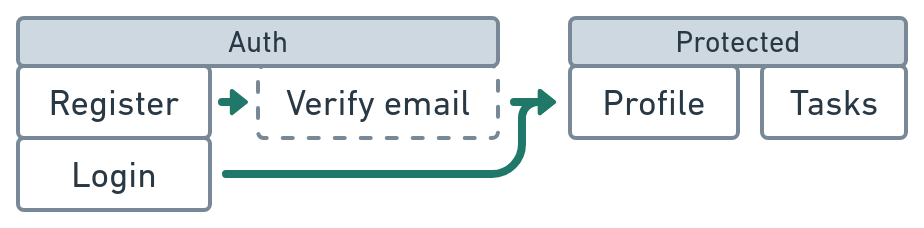
\includegraphics[width=0.5\linewidth]{images/ui-all.png}}
\vspace{-5pt}
\caption{Navigation flow for all users}
\label{fig:ui-all}
\vspace{-20pt}
\end{figure}
Figure \ref{fig:ui-all} represents the general navigation we want all users to take. The grey cells represent the parent route, which will appear in the url, and the white cells may be a component, or child route. The reason for a shared auth route is that we can have one page have a login and register form without a page redirection. Verify email will actually be a child route with the sole purpose of verifying and redirecting the user. 

The protected route is where all other pages will be. SvelteKits server hook will require all users to be authenticated through the Django API before they can access any pages - the most basic security measure. A common decision is to put authentication inside \texttt{+layout.server.ts}, as it encompasses all other routes after all. However, this is a massive security risk, as even unauthenticated uses can access the data fetched from the database. This is because the layout load function runs in parallel with the page's load function, so even if an unauthenticated user is redirected, the layout may still fetch data from the database. This isn't the only risk, for example if a user logs out in one tab, but keeps another tab open on a page that requires authentication, refreshing the second tab would bypass the authentication check because the layout's load function would not be aware that the user is no longer logged in.

All users will be initially redirected to the Profile page, which is to encourage keeping accurate records as they will see them every time the log-in. These records are important as they are automatically sent alongside forms that the user would otherwise have to fill out every time. They also have a Tasks button, which will automatically list all JDs and AACs that require action in one place.

\begin{figure}[h]
\centering
\frame{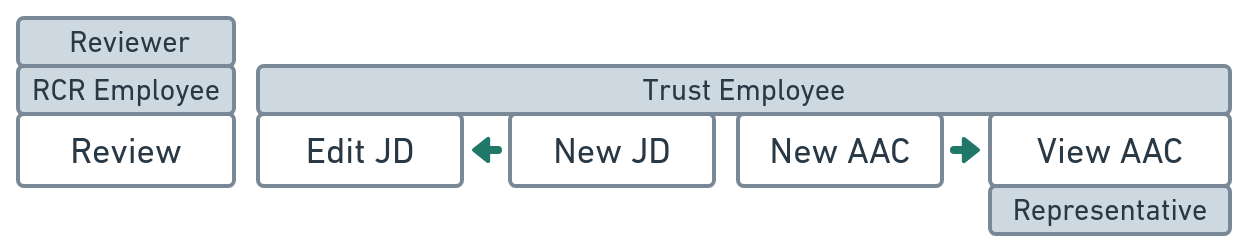
\includegraphics[width=0.75\linewidth]{images/ui-role.png}}
\vspace{-5pt}
\caption{Navigation flow for specific users}
\label{fig:ui-role}
\vspace{-5pt}
\end{figure}

Figure \ref{fig:ui-role} represents the navigation flow for specific users. The white cells represent buttons in the nav-bar. The process technically starts at different stages for all users, however they all depend on a JD. A Trust Employee will start by clicking the New JD button in the nav-bar, and is redirected to that page. Once submitted, they are automatically redirected to the Edit JD page, which also has its own button. This page will display information about the JD, and provide a form for the Trust Employee to complete. This form will include a dynamic amount of questions, dependent on the consultant type of the JD, and answer fields for content such as page numbers and general comments. Navigation to the Edit JD page through a button will present a list of still editable JDs specific to that user which can be edited at any time.

Once saved, the next step is to be completed by the RCR Employee, who will have the same page as the Trust Employee, but with an added row for comments. Of-course, just like Edit JD, they are first presented with a list of JDs that require review. The RCR Employee will be able to save their changes, and submit or reject when they are ready. When submitting, they will be given a list of Reviewers they can send the JD to with relevant information, in order to help chose the best option. Reviewers will have the same page, but again with an added row for comments. 

Once a JD is approved, the Trust Employee will be able to click the New AAC link to create a new panel. They will be able to select as many JDs as they like from a list, along with the date of the panel. They will then be redirected accordingly to View AAC. This page will have a list of valid Representatives along with contact details, in order of suitability. The Trust can choose one Representative, who will be given access to that AAC. Either the Trust or Representative can then download and upload an Outcome Form, which will be sent to the RCR Employee for data analysis. The reason this step is not a form is that interview outcomes are sometimes written by hand, or in person, where a Doctor may prefer not to use a computer.

\clearpage
\section{Coding Style}
The following style choices are personal preferences, with some influence from conventions. 

PEP 8 \parencite{guido_van_rossum_pep_2013} will be followed for all python code, more specifically, Black, and this style will be kept the same for variables passed from Django to SvelteKit. New variables and functions defined in SvelteKit will use camel-case in line with JavaScript conventions. A deviation from PEP 8 is that comments will be avoided as much as possible. This encourages code that is self-explanatory, such as descriptive variable and function names, and smaller easy to follow algorithms. It removes the risk of comments, which are subjective, being misinterpreted or outdated. There are exceptions, such as complex code that performs a task that is not immediately obvious.

Nested code in Python will be limited to a maximum of three layers of indentation. This practice helps reduce the cognitive load on the programmer. As aptly put by \textcite{the_kernel_development_community_linux_2024}:

\begin{displayquote}
"If you need more than 3 levels of indentation, you're screwed anyway, and should fix your program."
\end{displayquote}

\vspace{1em}
In Django we can also avoid the fat models design since we have a service layer. This common idea violates the Single Responsibility Principle (SRP) and makes code hard to read as the models become huge \parencite{martin_agile_2003}. Functions in models will be limited to essential methods such as \texttt{\_\_str\_\_} and \texttt{Meta}, \texttt{\_\_init\_\_}, and potentially \texttt{save}. 

In SvelteKit, HTML will be separated into components to keep the number of lines in a file short, and allow component reusability. Linting will be used with ESLint to enforce a consistent style across all files, and to catch errors early.